\chapter{Diseño e implementación de los sistemas SL y SL mini}

En este capítulo se detallará cuál es el hardware utilizado para el desarrollo del sistema de acceso, se indicarán cuáles
son los requisitos mínimos que deben satisfacerse para que el sistema cumpla las características solicitadas, como
también se indicarán los sensores y equipos auxiliares usados junta con otras posibles opciones encontradas y las
razones por las que estas fueron descartadas.


\section{Análisis de requisitos}


\subsection{Sistemas actuales}

Los sistemas más utilizados son por tickets, y por radiofrecuencia.

\subsubsection*{Sistemas tradicionales de tickets}

Este sistema de control de ingreso y egreso suele generar molestias en muchos de los usuarios, por la necesidad de realizar alguna acción extra, como presionar un pulsador para obtener y guardar un ticket con los datos de entrada este sistema se puede apreciar en Fig. \ref{fig:sistema-tradicional}.
Los tickets poseen un gran inconveniente, ya que si el usuario los pierde se le cobra un valor fijo, que en general es mayor al tiempo de la estadía.
Estos sistemas cuentan con el inconveniente de que la impresión del ticket se realiza por impresión térmica, lo que requiere un papel termosensible.
Otro inconveniente de este sistema es el impacto ambiental del de la emisión de papeles de un solo uso. En promedio un usuario tarda entre 10 y 15 segundos en entrar o salir del establecimiento.

A continuación sé listas las desventajas de este sistema:

\begin{enumerate}
    \item Tiempo de acceso.
    \item Emisión de papeles de un solo uso.
    \item Necesidad de acciones por parte del usuario.
\end{enumerate}

\begin{figure}
    \centering
    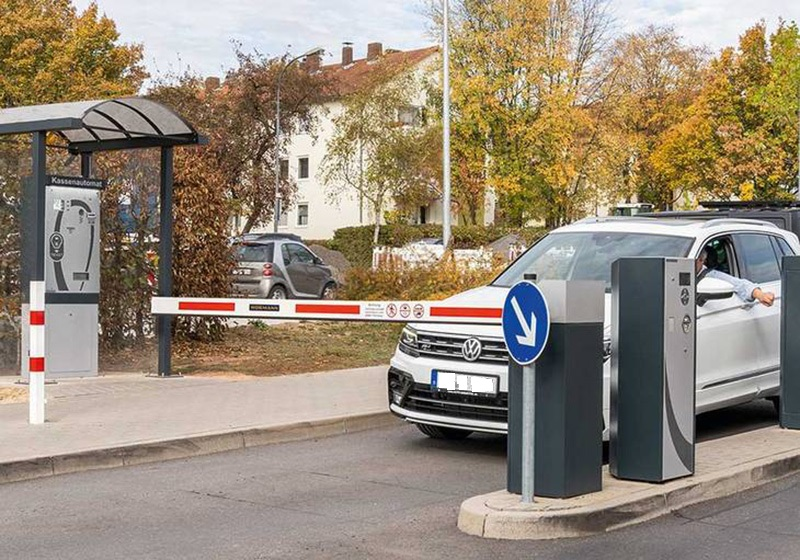
\includegraphics[width=0.5\textwidth]{imgs/sistema-control-acceso-barreras.jpg}
    \caption{Sistema tradicional de acceso por barreras.}
    \label{fig:sistema-tradicional}
    %%https://www.aradock.es/nuevos-sistemas-de-control-de-accesos-barreras/
\end{figure}

Otro de los aspectos que destacan del uso actual del sistema de barreras en sistemas más manuales es la necesidad de
contar con  operarios trabajando en la barrera el tiempo que la barrera esté disponible, ya que en caso de no disponerlo
deberá quedar la barrera sin efecto, perdiendo por completo su utilidad.

\subsubsection*{Sistemas de radiofrecuencia}

Con el avance y el abaratamiento de los costos en la electrónica surgieron nuevos métodos que permitieron a los usuarios prescindir de la necesidad de un ticket o una tercera persona que les facilite el acceso, el método principal es el uso de controles remotos que al ser accionados, activan el mecanismo y abren el paso del vehículo.

Otro sistema que está ocupando gran parte del mercado en los últimos años es el que integra a la barrera un sistema de RFID, que mediante la colocación de un emisor RF en el vehículo, Fig.\ref{fig:sistema-moderno} o por el método de tarjetas o monedas de proximidad y un receptor en la barrera, al acercarse al ingreso se produce en el enlace que habilita o no al vehículo a ingresar. La gran desventaja de este sistema es tener que instalar el emisor RF en el vehículo o guardar la tarjeta de lectura.

Los problemas de este sistema son:

\begin{enumerate}
    \item Necesidad de instalar un emisor RFID.
    \item Distancia de actuación corta.
\end{enumerate}

\begin{figure}
    \centering
    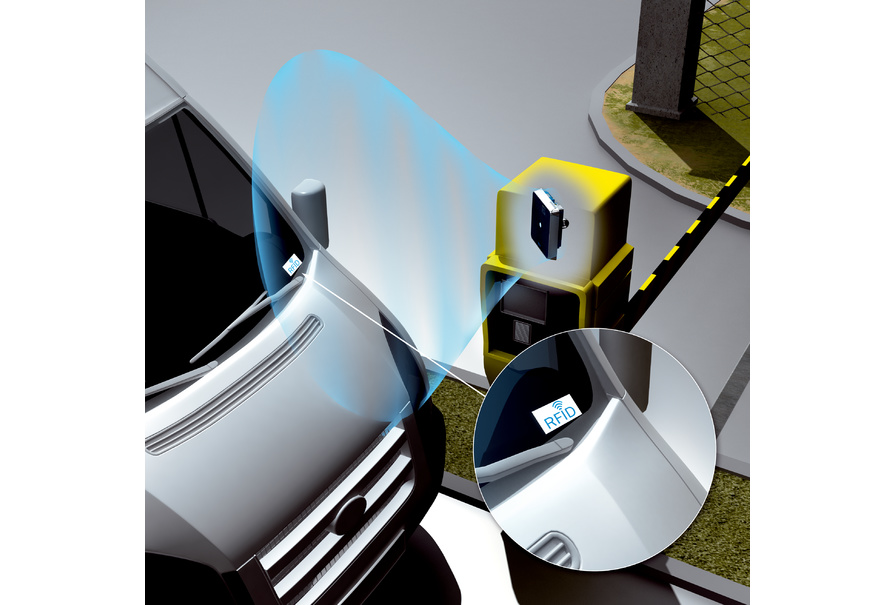
\includegraphics[width=0.8\textwidth]{imgs/sistema-control-acceso-barreras-rfid.jpg}
    \caption{Sistema moderno de acceso por barreras por sistema de RFID.}
    \label{fig:sistema-moderno}
    %%https://www.sick.com/mx/es/sectores/seguridad-de-los-edificios/seguridad-en-los-exteriores/control-de-acceso/acceso-sin-contacto-a-barreras-mediante-rfid/c/p360565
\end{figure}

\subsection{Requisitos de los sistemas SL}

Los métodos anteriormente nombrados son muy útiles en el día a día, pero cuentan con una serie de inconvenientes que pueden ser atenuados mediante el OCR, ya que se utiliza un distintivo único de los autos, como es el sistema de RFID, la distancia de actuación está dada por la distancia máxima de reconocimiento del algoritmo, y los sensores empleados.

Debido a la necesidad de realizar OCR, se requerirá una cámara. Con la finalidad de poder acoplar algún sistema de activación para la cámara se exigirá que la placa elegida soporte protocolos como I2C, SPI y UART. En cuanto a la comunicación, como se implementara junto con un servidor web existe la necesidad de conexión Ethernet o Wifi. Finalmente para facilitar futuras actualizaciones se requiere que la placa pueda correr un sistema operativo basado en GNU/Linux.

En resumen los requerimientos son:

\begin{enumerate}
    \item Implementación de una cámara.
    \item Soporte a protocolos I2C, SPI, UART.
    \item Conexión Ethernet o Wifi.
    \item Tiempo de acceso menor a 10 segundos.
    \item Sistema operativo basado en GNU/Linux.
\end{enumerate}


\section{Selección de placas}

Teniendo en cuenta los requisitos planteados en la sección anterior, se presentan varias opciones posibles,
placas de la empresa Raspberry Pi, embebidos de la serie STM32 e incluso placas de la marca Arduino en sus versiones más potentes, por nombrar las más conocidas.
Aquí es donde surge el primer inconveniente para tomar la elección de placa,
cuál sería la mejor opción que cumpla tanto las necesidades y que sea accesible para poder realizar el proyecto.
Luego de realizar una investigación de placas a las que se podía acceder se optó por 2 modelos basados en una Raspberry Pi 3 B+ a la cual se la llamo SL mini, y la otra basada en una NVIDIA Jetson TX1 denominada SL.

\subsection{Características del SL mini}

La placa de la barrera SL mini es una Raspberry Pi 3 B+, Fig. \ref{fig:raspberry} la cual cuenta con un procesador
Broadcom BCM2837B0 y un Córtex A53 acompañado de 1 GB de RAM LPDDR2, junto con un sistema operativo llamado Raspberry Pi OS el cual está basado en Debian.

\begin{figure}
    \centering
    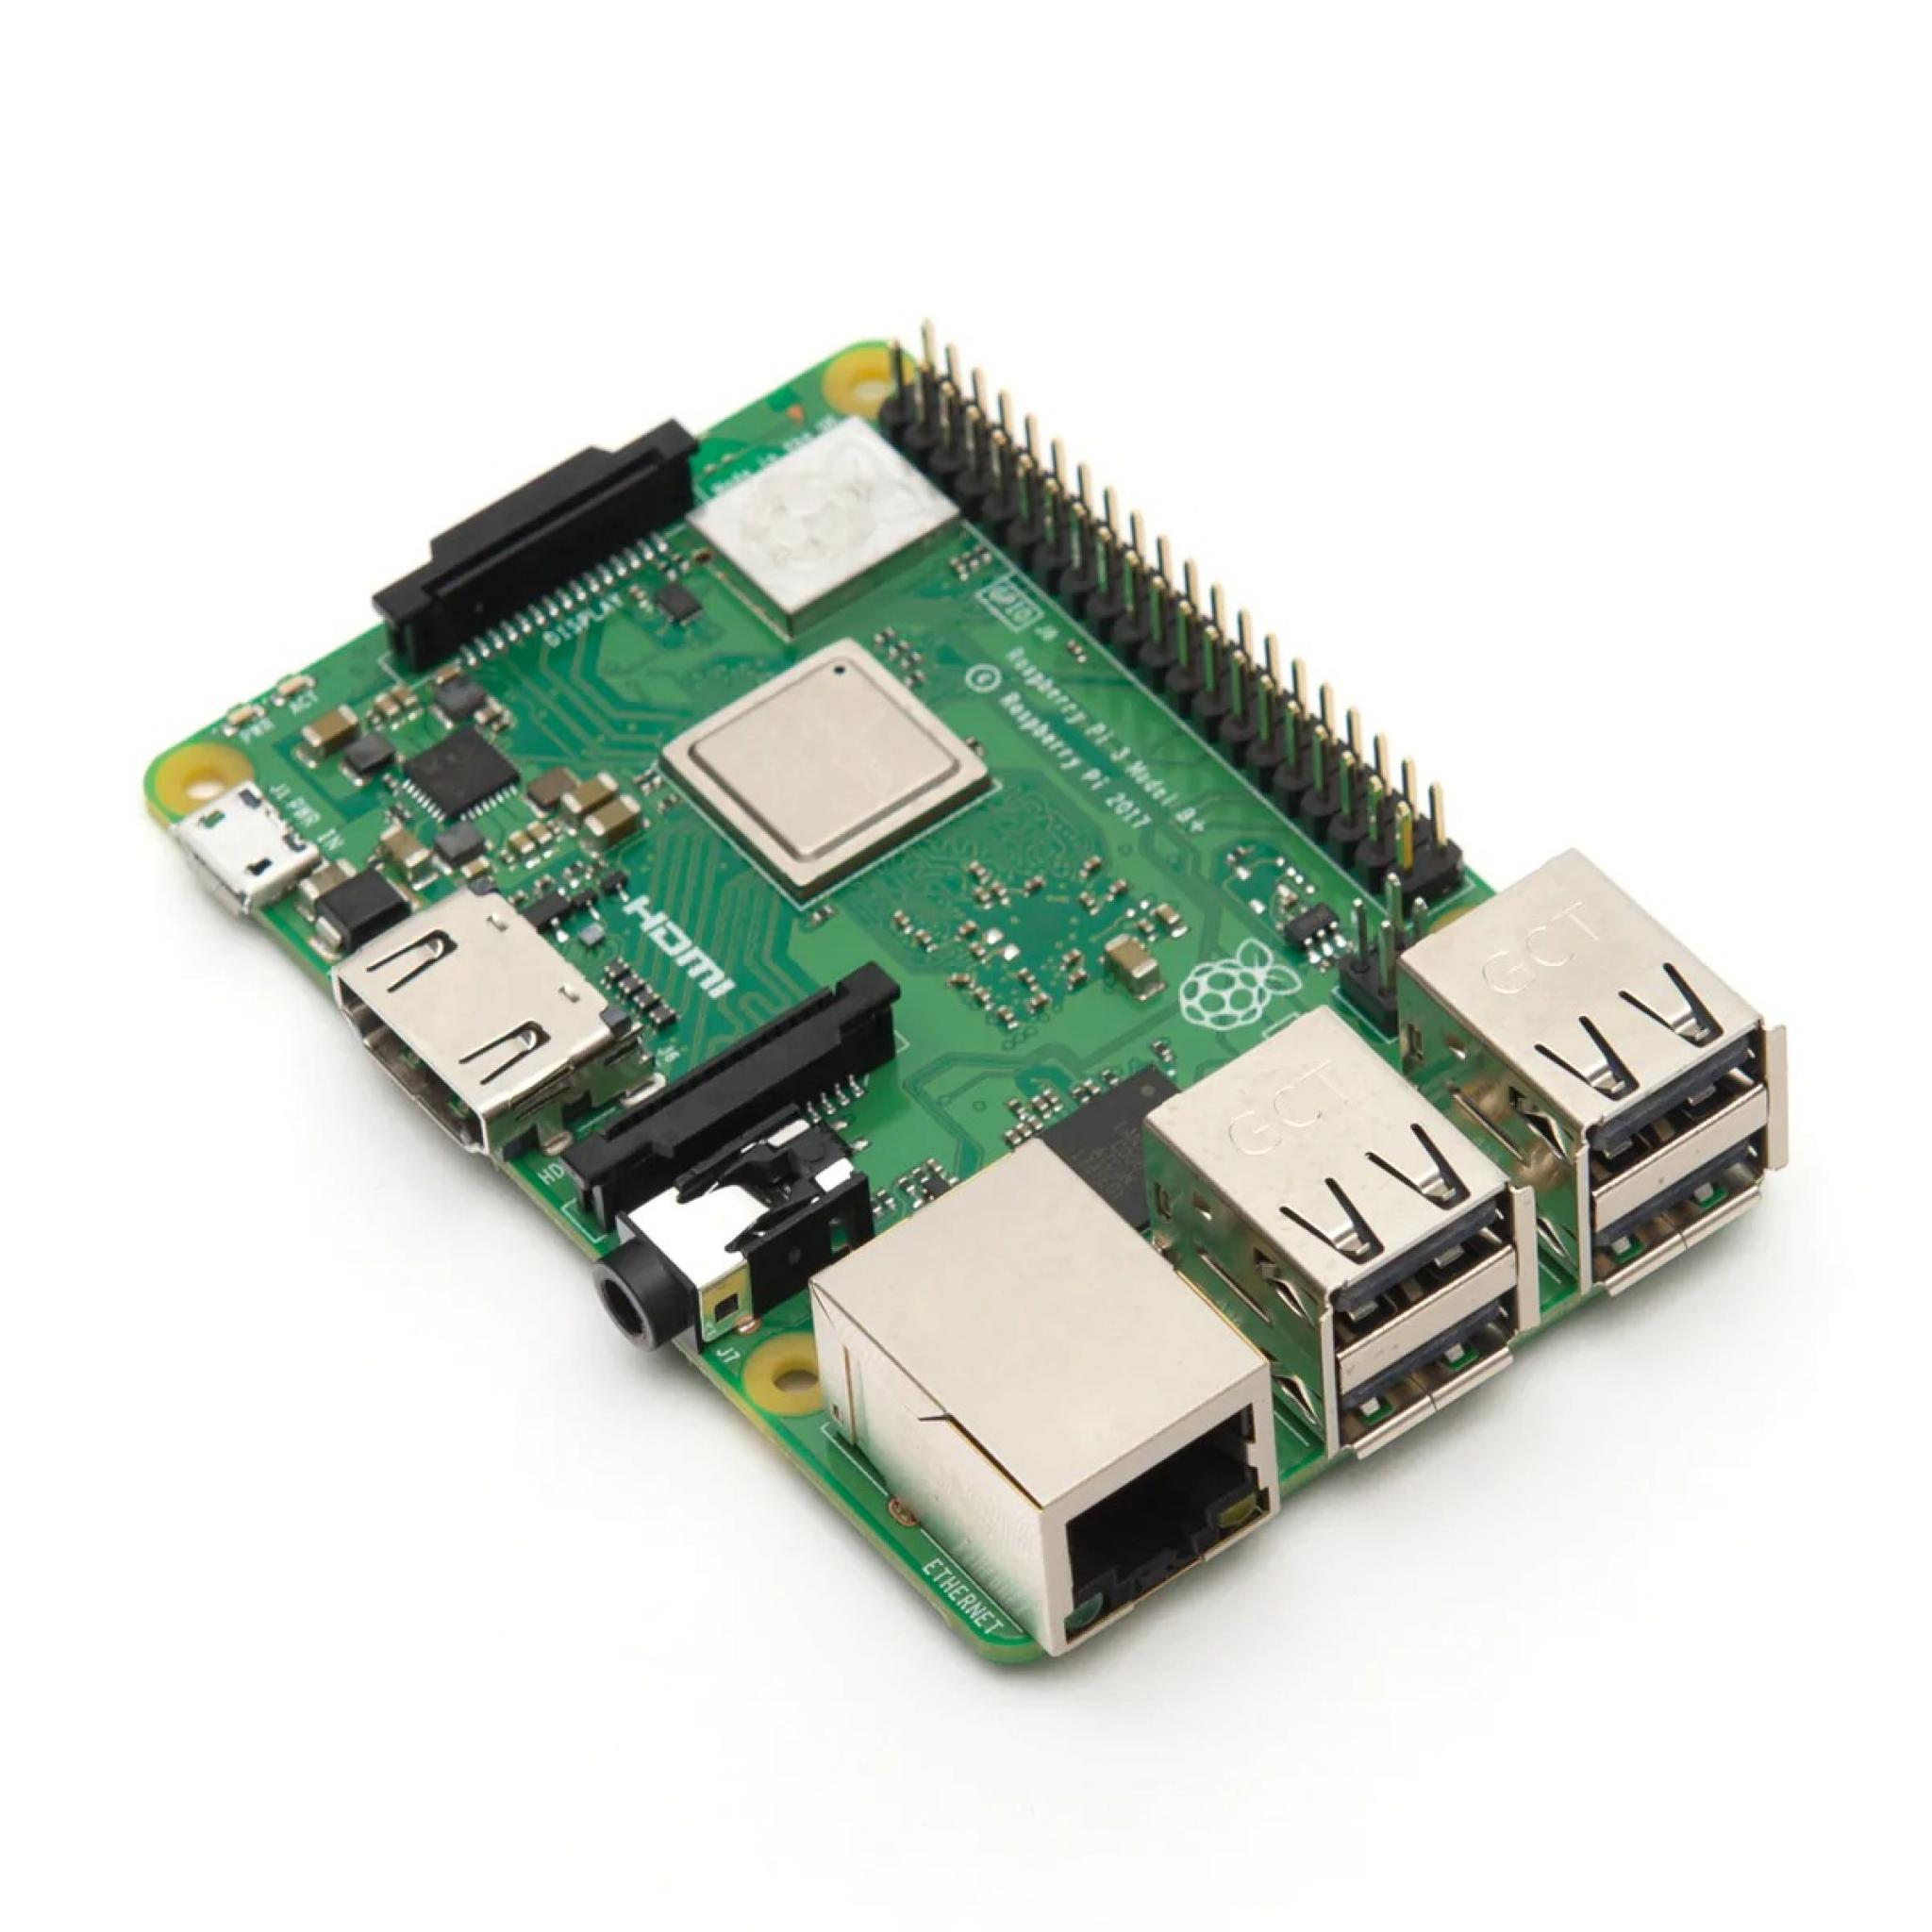
\includegraphics[width=0.4\textwidth]{imgs/Raspberry-pi3b+.jpg}
    \caption{Raspberry Pi 3B+.}
    \label{fig:raspberry}
\end{figure}

Otro de los puntos importantes que destacan de la placa son los pines GPIO, pines de entrada/salida de propósito general por sus siglas en inglés, lo que la hace sumamente sencilla a la hora de utilizarla junto a sensores comerciales.
La amplia conectividad integrada que posee fue un punto que la destacó sobre otras posibles placas de desarrollo, ya que cuenta con puertos de conexión USB 2.0, puerto Ethernet, conexión Wifi 2,4 y 5,8 GHz y comunicación Bluetooth 4.2, suple la necesidad de brindar conexión a internet de manera nativa sin necesidad de contar con periféricos extras que puedan encarecer el sistema.

La disponibilidad de la placa en el mercado, fue un punto importante a considerar, ya que pensando en una futura
implementación del sistema a mediana o gran escala o la necesidad de cambio por rotura de la misma, podían dejar el
proyecto parado o inutilizado generando otros inconvenientes. Por otro lado, es posible migrar a un modelo más nuevo como la versión 4, sin tener que realizar grandes cambios en los drivers diseñados.

Si bien las capacidades de la Raspberry son amplias, para este proyecto su poder de cómputo no fue suficiente para realizar por sí misma el procesamiento de la imagen en un tiempo menor a 10 segundos, ya que demora un aproximado de 1:30 minutos, tiempo que se consideró excesivo.

\subsection{Características del SL}

La placa de la barrera SL es una Nvidia Jetson TX1, Fig. \ref{fig:JTX1} la cual cuenta con un procesador Córtex A57, además de contar con 256 núcleos Nvidia Maxwell, lo que la vuelve una opción excelente en lo que se refiere al trabajo con imágenes y videos, junto a 4GB de RAM LPDDR4, la hacen una opción mucho más potente en capacidad de cómputo que la Raspberry Pi 3 B+.

Para realizar la implementación se contó con el kit de desarrollo provisto por la empresa Nvidia, en él se pueden encontrar todas las conexiones mencionadas en la barrera SL mini, lo que permite el paso de los sensores de una placa a otra con suma facilidad.
Este modelo cuenta con un sistema operativo JetPack 4.6.3 basado en Ubuntu 18.04.

\begin{figure}
    \centering
    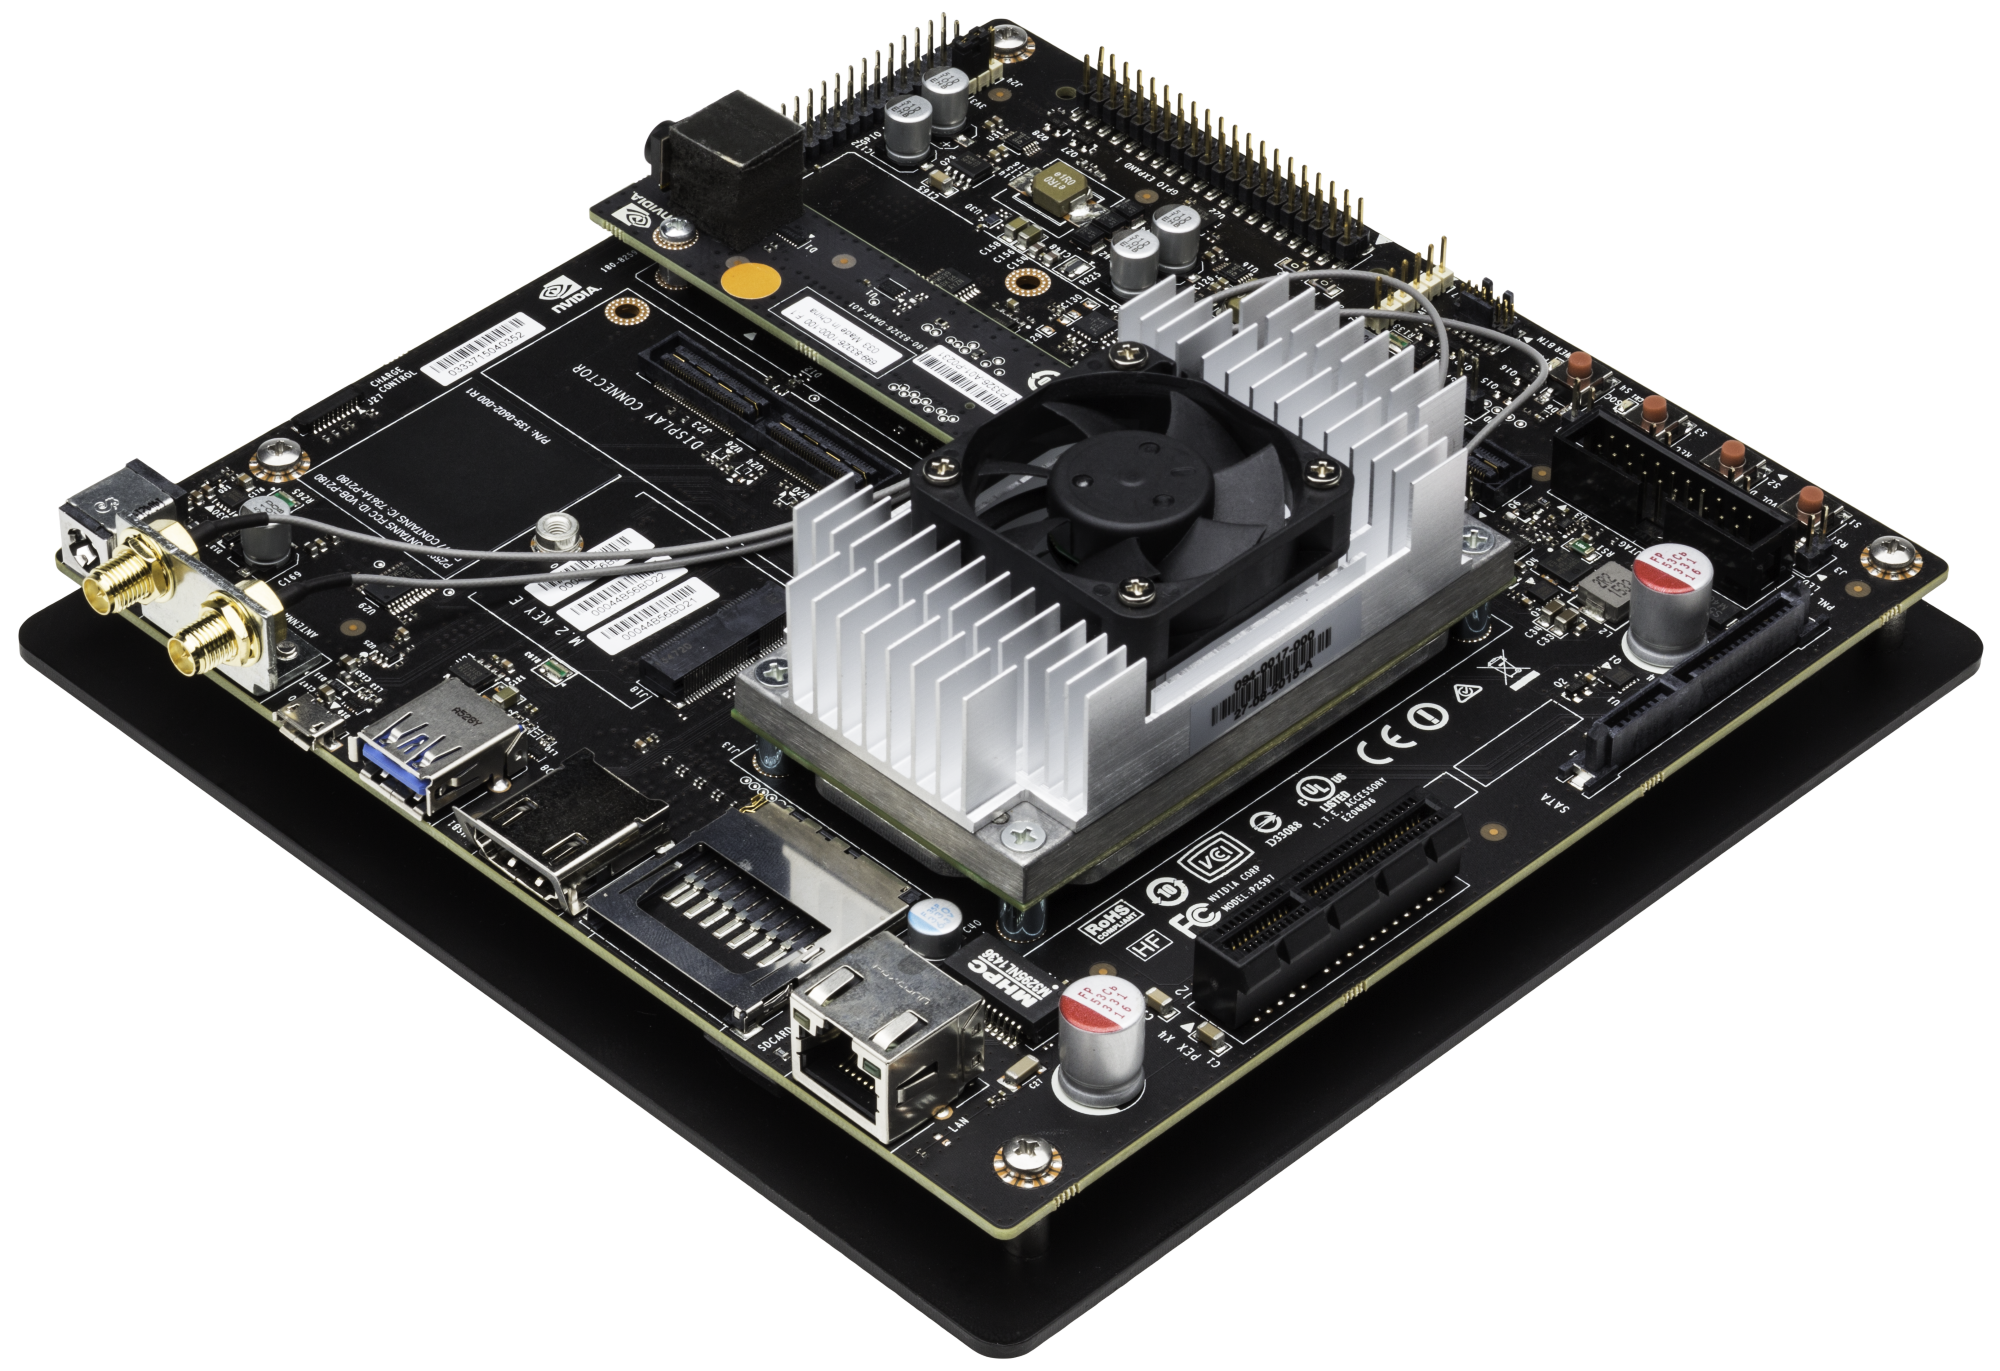
\includegraphics[width=0.3\textwidth]{imgs/JTX1-developerkit.png}
    \caption{Nvidia Jetson TX1 developer kit.}
    \label{fig:JTX1}
\end{figure}


En contra parte con el modelo mini, la placa del modelo SL está pensada para el trabajo con redes neuronales y el manejo de imágenes, por lo que es posible integrar todo el sistema de reconocimiento de caracteres dentro del mismo algoritmo embebido en la placa, teniendo un tiempo de respuesta de aproximadamente unos 6 segundos, tiempo que se consideró aceptable.

\section{Evaluación y selección de sensores}

En este apartado se estudiara la evalución del sistema de actuación

\subsection{Selección de cámara}
Si bien tanto el modelo de placa SL como su versión mini aceptan cámaras con conexionado propio provistas por las empresas que las crearon,
se tomó la decisión de utilizar una cámara web con conexión USB, Fig. \ref{fig:camara-usb}, se utilizó un modelo genérico, comprada vía Mercado
Libre, ya que estas no requieren de drivers complementarios para funcionar, es decir son Plug and Play, son fácilmente reemplazables
por otro modelo en caso de rotura o simplemente cambiarla por otra que sea de mejor resolución de imagen, además de poseer un precio reducido,
comprada con otro tipo de cámaras USB u orientadas al uso en domótica.
\begin{figure}
    \centering
    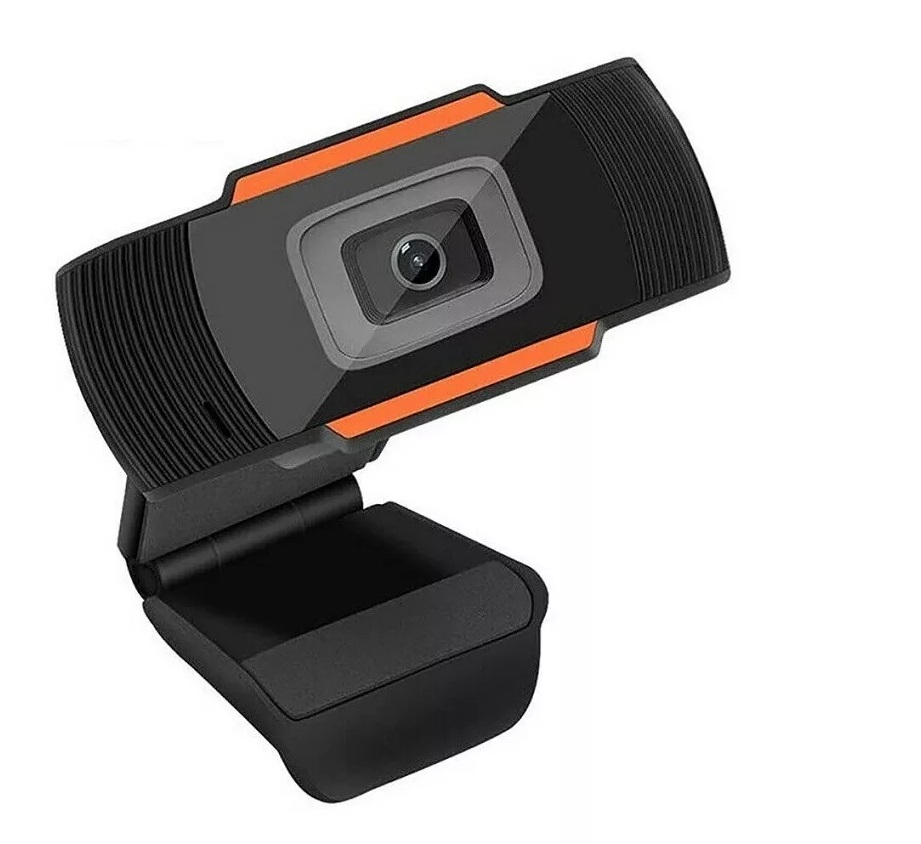
\includegraphics[width=0.5\textwidth]{imgs/camara-usb.jpg}
    \caption{Cámara utilizada.}
    \label{fig:camara-usb}
    %https://www.mercadolibre.com.ar/camara-webcam-para-pc-microfono-usb-720p-hd-windows-10/p/MLA21775903#searchVariation=MLA21775903&position=2&search_layout=stack&type=product&tracking_id=8191aaa4-4b06-41e0-b681-ded2c4d4b641
\end{figure}

\subsection{Selección de activador}
Una vez que nos decidimos en la cámara, fue hora de analizar como decirle al sistema que obtenga la imagen, analizamos como suelen funcionar
algunos sistemas que requieren que un objeto se aproxime o cruce un espacio específico y encontramos estas posibles opciones:

\begin{itemize}
    \item Barrera infrarroja: mediante la utilización de un haz de luz infrarroja se indice sobre un receptor, por  lo cual al acercar el vehículo a
          la barrera el haz se ve interrumpido generando un cambio en el receptor que accionaria la cámara. Este mecanismo cuenta con varios inconvenientes
          como la sensibilidad del receptor a la radiación infrarroja del ambiente, la posible interrupción del haz por suciedad (recordando que el
          sistema puede encontrarse a la intemperie), entre los  más destacados. Este método fue uno de los más probados por nosotros, en primera instancia
          fabricamos una barrera infrarroja, pero no contaba con el alcance para permitir que un vehículo la atraviese, y las opciones comerciales, excedía
          los costos que nos parecían razonables para invertir en este apartado. Por estas razones fue que el uso de una barrera infrarroja fue descartado.

    \item Placa de presión: un sistema simple que usa una placa sobre el terreno que al ser pisada por el vehículo
          genera una señal de activación, el inconveniente se encuentra en la instalación de la plancha, debido a que no todos
          los accesos tienen la capacidad de permitirlo, por lo que esta opción se descartó.

    \item Sensores capacitivos: estos generan campos magnéticos que en presencia de objetos se ven afectos, con lo
          que con una calibración correcta podría ajustarse para detectar vehículos, la difícil adquisición de los mismos por falta de stock, por costos o
          dificultad para crearlos llevaron a descartar esta opción.

    \item Sensores ultrasónicos: Estos miden la distancia mediante la emisión de una onda ultrasónica por un transmisor y
          mediante el tiempo que tarda la onda emitida en llegar a un receptor se estima la distancia. Esta fue la opción elegida, ya que es una opción
          de un costo no muy elevado, relativa facilidad de integración a diversas placas embebidas y cuenta con la ventaja de tener una variedad de modelos
          disponibles en el mercado que se adaptan a los diferentes protocolos de comunicación.
\end{itemize}
El sensor elegido para el diseño de ambos prototipos fue el sensor ultrasónico US-100,Fig. \ref{fig:sensor-US100}, el cual permite un
rango de medición de 2 cm a 350 cm, compensado por temperatura, voltaje de alimentación entre 3V-5V y protocolo de
comunicación UART. Por lo que es integrable a ambas placas por medio del puerto GPIO sin necesidad de requerir de conversores de nivel lógico
ni hardware de alimentación adicional.
\begin{figure}
    \centering
    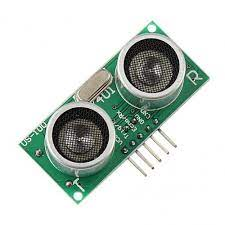
\includegraphics[width=0.5\textwidth]{imgs/us-100.jpg}
    \caption{Sensor US-100 usado en los prototipos.}
    \label{fig:sensor-US100}
\end{figure}

\section{Consumo energético}

El gasto energético es un punto que fue analizado, ya que, pensando en el uso racional de la energía, queríamos que nuestros prototipos no
presentaran un consumo excesivo, y que en un futuro si alguien lo deseaba sean alimentando por un panel solar junto con una batería.
Como la energía suministrada al conjunto cámara-sensor viene dada por las placas, solo se indicara el consumo requerido por las placas SL y SL mini.
\subsection{Consumo energético Modelo SL}

El requerimiento energético previsto por el fabricante para el kit de desarrollo de la Nvidia Jetson TX1 como se indica
en el cargador que viene dentro del kit es de 19 volts y 4,74 ampers (máximo 90 Watts).

Lo que podría ser alimentado con el uso de una batería de 12 volts o 24 volts y un algún circuito externo que regule la
tensión a los 19 volts solicitados, siempre y cuanto este sea capaz de suministrar la corriente necesaria.

\subsection{Consumo energético Modelo SL mini}

En el caso de la versión SL mini, tiene un consumo similar al de un cargador de celular moderno, es decir unos 5 volts y
2 ampers, ya que una corriente menor lleva a una notificación por parte de la placa, indicando que la energía no es la
suficiente reduciendo la frecuencia de su procesador, ralentizando el equipo.

Este consumo reducido es fácilmente lograble con un sistema de carga de celular portátil, por lo que sería más sencillo
alimentarlo en caso de no disponer una toma de corriente de la red doméstica.

\section{Diseño y ensamble}

Para la colocación del conjunto de prueba cámara-sensor, se diseñó e imprimió un contenedor en 3D,Fig. \ref{fig:contenedor-camara}
que sera soportado por un trípode o puede ser anclado a una pared o poste cercano a la zona de acceso.
\begin{figure}
    \centering
    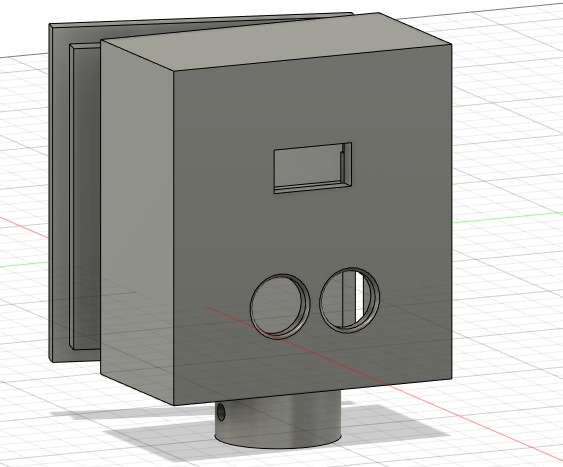
\includegraphics[width=0.5\textwidth]{imgs/contenedor-camara.png}
    \caption{Modelo 3D del contendor del paquete cámara-sensor.}
    \label{fig:contenedor-camara}
\end{figure}

Al tratarse de un prototipo se buscó que el diseño sea lo más simple posible, permitiendo ser fácilmente modificable, en el caso de necesitar
modificarlo en un futuro, ya sea por cambio de hardware o una necesidad de un punto de colocación diferente.

Se optó por colocar el sensor de proximidad en la zona inferior, ya que el ideal es colocar el contenedor a una altura de unos 60 cm
aproximadamente, con lo que al tener el sensor en la zona baja se garantiza que la lectura que se tome sea de la trompa del automóvil y se
obtenga un valor certero de la distancia.

Esto deja a la cámara en la zona superior del contendor dando una imagen lo más completa de la trompa del vehículo, tomando así la vista
completa de la patente, esto con el fin de evitar que la patente salga recortada impidiendo que esta sea reconocida por el algoritmo.

Se dispuso un orificio en la zona inferior de la caja con la finalidad de colocar un eje, que permita la orientación del dispositivo, dependiendo
el lugar donde se desee instalarlo, para la sujeción al eje se realizaron 2 pequeños orificios que permitan el paso de 2 tornillos que dejen fijo
el contenedor al eje.
\begin{figure}
    \centering
    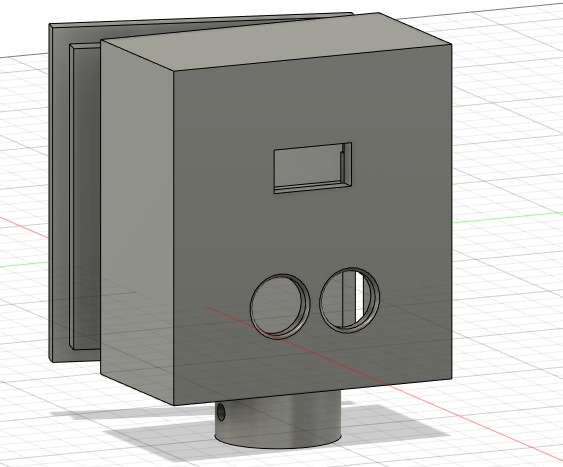
\includegraphics[width=0.5\textwidth]{imgs/contenedor-camara.png}
    \caption{sistema de sujeción del contenedor.}
    \label{fig:sujecion-contenedor}
\end{figure}

En la Fig. \ref{fig:contenedor-camara-real} se puede apreciar el contenedor ya con la camara y el sensor instalados.

\begin{figure}
    \centering
    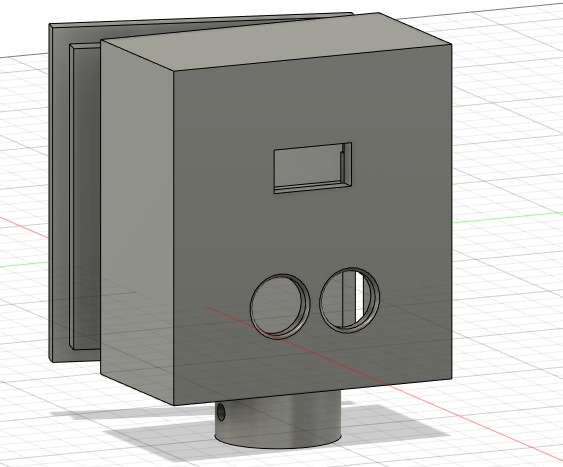
\includegraphics[width=0.5\textwidth]{imgs/contenedor-camara.png}
    \caption{Contendor del paquete cámara-sensor.}
    \label{fig:contenedor-camara-real}
\end{figure}

